\documentclass[../psets.tex]{subfiles}

\pagestyle{main}
\renewcommand{\leftmark}{Problem Set \thesection}
\setcounter{section}{2}
\setenumerate[2]{label={\alph*)}}

\begin{document}




\section{PCR, Sequencing, Cell Structure, and Localization}
\begin{enumerate}
    \item \marginnote{11/29:}PCR.
    \begin{enumerate}
        \item Can you describe a way to amplify a strand of RNA (i.e., make a large number of [DNA or RNA] copies so that you can submit it for sequencing, for example)? But your challenge is to achieve this using any enzyme (or set of enzymes) except a DNA polymerase. (4 pts)
        \item Professor Tang has invented a new DNA polymerase that produces 3 DNA strands every time it copies a template strand. After 10 cycles of PCR, on a target segment she amplified, how many target DNA strands will she have in the mixture? How many variable length strands will she have in the mixture? 2 bonus points for a mathematical rationale. ($4+2$ pts)
    \end{enumerate}
    \item Sequencing.\par
    In Maxam-Gilbert sequencing, the 4 nucleotides A, T, G, and C react in 4 specific reactions, leading to the strand being cleaved when it is treated with hot piperidine. For each nucleobase, write below the chemical reaction that occurs, and how the strand gets cleaved. Hefty bonus points for the reaction mechanism. ($4\times 1$ pt for the reaction; $4\times 2$ pts for the reaction mechanism)
    \item Sequencing primer.\par
    Assuming the sequence of the human genome is completely random (it is not!), what is the minimum length of DNA primer you would need for it to bind only to a single site in the human genome? The number alone is invalid, unless accompanied by a calculation. (4 pts)
    \item Plasma membrane and cell structure.
    \begin{enumerate}
        \item When a lipid bilayer snaps or breaks, why can it not repair itself by forming a hemi-micelle cap as shown in the figure below? (4 pts)
        \begin{figure}[h!]
            \centering
            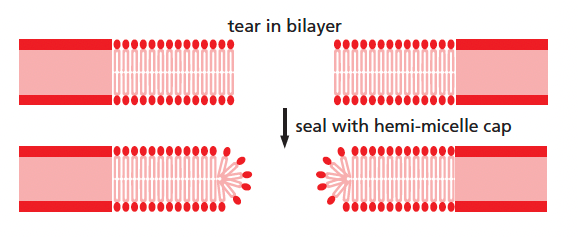
\includegraphics[width=0.4\linewidth]{../ExtFiles/pset3-hemiMicelle.png}
            \caption{Hypothetical hemi-micelle membrane repair.}
            \label{fig:pset3-hemiMicelle}
        \end{figure}
        \item You are studying the binding of proteins to the cytoplasmic face of tumor associated macrophages for which you need a pure population of "inside-out vesicles" made from the plasma membrane. You have devised a method that gives a good yield of inside-out vesicles from the plasma membrane, but your preps are still contaminated with varying amounts of right-side-out vesicles. A senior grad student in the lab suggests that you pass your vesicles over an affinity column made of lectin coupled to solid beads. What is the rationale underlying her suggestion? (3 pts)
    \end{enumerate}
    \item Protein export and import.\par
    Describe a strategy to position a fluorescent protein, say GFP, anchored to the inner mitochondrial membrane, but projecting into the intra-lumenal space. What are the steps that lie between the mRNA of this protein being translated, up until the protein is positioned as above? (7 pts)
\end{enumerate}




\end{document}